\documentclass[conference]{IEEEtran}
\usepackage[utf8]{inputenc}
\usepackage{cite}
\usepackage{amsmath,amssymb}
\usepackage{graphicx}
\usepackage{booktabs}
\usepackage{subcaption}
\usepackage{url}
\usepackage{microtype}
\usepackage{multirow}
\usepackage{enumitem}
\usepackage{algorithm}
\usepackage{algorithmic}
\usepackage[T1]{fontenc}
% If using hyperlinks in bibliography (optional)
\usepackage[hidelinks]{hyperref}

\begin{document}


\title{Detecting Adversarial Data Poisoning in Federated Learning\\
Using Independent Class-wise Coherence Score (ICS)}

\author{
  \IEEEauthorblockN{Laiba Mazhar}
  \IEEEauthorblockA{National University of Computer and Emerging Sciences\\
    Email: i221855@nu.edu.pk}
  \and
  \IEEEauthorblockN{Supervisor: Dr. Nouman Noor}
  \IEEEauthorblockA{National University of Computer and Emerging Sciences}
}


\maketitle

\begin{abstract}
Federated Learning (FL) enables collaborative model training across distributed clients without sharing raw data, strengthening privacy but exposing systems to adversarial data poisoning attacks where malicious clients manipulate local training data to compromise global model behavior. Existing defenses, including coherence-based approaches, assess client trustworthiness based only on global prediction agreement, failing to capture class-specific behaviors and lacking adversarial stress-testing capabilities. Consequently, these methods are ineffective against targeted label-flipping and backdoor attacks that subtly distort class-conditional decision boundaries. This paper proposes the Independent Class-wise Coherence Score (ICS), a novel defense mechanism that evaluates client reliability independently for each class using adversarially generated MI-FGSM probes. ICS computes four coherence metrics—Output Consistency, Class Confidence, Inverse Entropy, and Prediction Consistency—fusing them into a weighted score for selective aggregation. Evaluated on MNIST, EMNIST, and CIFAR-10 under targeted label-flipping attacks, ICS achieves 75.02\% accuracy with 19.75\% Attack Success Rate (ASR) on MNIST, outperforming global-coherence baselines by 5-7\% in accuracy while reducing ASR by 30-40\%. Similar improvements are observed across EMNIST and CIFAR-10. Ablation studies validate the necessity of each ICS component, demonstrating that ICS provides precise, adversarially-robust detection for FL security in real-world distributed environments.
\end{abstract}

\begin{IEEEkeywords}
Federated Learning, Adversarial Attacks, Data Poisoning, Coherence Score, MI-FGSM, Robust Aggregation
\end{IEEEkeywords}

\section{Introduction}
Federated Learning (FL) allows joint model training among distributed customers without the exchange of raw data, enhancing privacy but introducing systems to adversarial data poisoning attacks in which the bad clients can use local training information to influence the behavior of the global model. Current defenses, such as coherence-based methods, determine client trustworthiness solely by a global comparison of predictions, and do not reflect class-specific patterns or are not capable of stress-testing their adversarial behavior. Thus, they do not work well in resisting targeted label-flipping and backdoor attacks that cause subtle manipulation of class-conditional decision boundaries. In this paper, the authors introduce the Independent Class-wise Coherence Score (ICS) a new defense mechanism, which assesses client reliability on a case-by-case basis on each individual class, based on adversarially generated MI-FGSM probes. ICS calculates four measures of coherence (Output Consistency, Class Confidence, Inverse Entropy, and Prediction Consistency), which are amalgamated into a weighted value to be used to selectively aggregated. Under targeted label-flipping attacks, evaluated over MNIST, EMNIST and CIFAR-10, ICS has accuracy of 75.02 with 19.75% Attack Success Rate (ASR) on MNIST, which is 5-7 points higher than global-coherence baselines, and lowers ASR by 30-40 points. The same is seen in EMNIST and CIFAR-10. The need of each ICS component is verified by ablation studies that reveal that ICS achieves accurate, adversarially-robust detection of FL security in realistic distributed systems.

Federated Learning has become a scalable architecture that allows a large number of players to collaborate in training machine-learning models without having to share personal information. The client does not send all the datasets to a server but instead calculates local gradients and sends them to be aggregated\cite{bagdasaryan2020backdoor}. The privacy is greatly enhanced by this design, and it is especially important in such areas as healthcare, financial analytics, and mobile apps. However, there is also a very tangible security issue on the other side of this coin as the server cannot only have confidence in the honesty of every client, but also as to whether the information received is based on clean data that has not been spoiled. An adversarial player can silently poison his/her data or gradients in the course of local training and distort the global model.

Such adversarial data poisoning can have large-scale devastating consequences. A single attacker has the ability to either switch labels, inject incorrectly labeled samples, or generate poisoned gradients which draw a complete model to erroneous results. This carries grave safety-related risks on systems in the face of malware being dubbed as harmless, improper medical diagnoses, autonomous driving perceptions, or the collapse of industrial IoT models. In the case where a compromised model is present, the model may remain bad even when the attacker has left, and hence it is important to detect them early.

Researchers have suggested different malicious client detection strategies. To illustrate the point, Cucu et al. suggested a method of coherence-based evaluation of client reliability through examining their prediction consistency on a global scale. Although it is useful in the context of naive poisoning, this is inherently gap-prone: it does not give preference to classes, does not reflect on the inconsistencies of classes, and does not understand that a model is robust to adversarial pressure. Numerous methods of poisoning, in particular targeted types of label-flipping and backdoor triggers are apparent at the class level, and thus global metrics fail to capture these hidden variations. Moreover, adversarial examples have been demonstrated to be very effective at exposing weak or malicious decision boundaries, but existing FL trust systems rarely involve adversarial probing\cite{ovi2025robust} 

In order to achieve this inadequacy, this paper proposes Independent Class-wise Coherence Score (ICS)-a finer-granular reliability indicator at the class level guided by adversarial signals. ICS builds MI-FGSM adversarial probes on each class and examines how customers respond on multiple coherence measures with increased identification of bad actors. In contrast with single, global coherence score, ICS identifies targeted attack on the basis of internal consistency of decision at the class level.

The significant contributions made by this work are:

\begin{enumerate}[leftmargin=*]
  \item A novel per-class coherence scoring mechanism (ICS) incorporating adversarial probing;
  \item A set of four coherence metrics—Output Consistency, Class Confidence, Inverse Entropy, and Prediction Consistency, combined into an interpretable weighted score;
  \item A selective aggregation strategy that leverages ICS for robust model updates;
  \item Comprehensive evaluation across MNIST, EMNIST, and CIFAR-10 under targeted poisoning;
  \item An extensive ablation study validating the necessity of each ICS component.
\end{enumerate}
The remainder of the paper is organized as follows. Section~\ref{sec:related} reviews recent work on FL poisoning and detection. Section~\ref{sec:gaps} outlines research gaps. Section~\ref{sec:method} presents the proposed ICS methodology. Section~\ref{sec:exp} details the experimental setup. Section~\ref{sec:results} reports and analyzes results. Section~\ref{sec:usecase_scenario} introduces a real-world use case and case study. Section~\ref{sec:comparison} compares the proposed method with prior work. Section~\ref{sec:conclusion} concludes the paper.
\section{Related Work}
\label{sec:related}

This section summarizes the work done regarding poisoning and backdoor attacks on FL, defenses based on robust aggregation and coherence, adversarial-example verification, and survey-level treatments related to FL security.

\subsection{Poisoning and Backdoor Attacks in FL}
Several works illustrate the effectiveness and persistency of poisoning and backdoor attacks against FL. Bagdasaryan et al. have proven that one malicious client could implant persistent backdoors using carefully constructed gradient updates \cite{bagdasaryan2020backdoor}. Xie et al. have analyzed the issue of targeted label-flipping attacks and shed light on how class-specific vulnerabilities can be targeted under federated aggregation \cite{xie2021targeted}. Zhao et al. assessed distributed poisoning in mobile FL and discussed the scalability of such an attack in edge environments \cite{zhao2023distributed}. Most recently, Wang et al. have analyzed fine-grained class corruption and argue that class-aware defenses should be developed to counteract subtle per-class manipulations \cite{wang2024class}.

Recent advances in 2025 have further highlighted the severity of poisoning attacks. Ovi and Gangopadhyay proposed robust federated learning mechanisms for prevention and detection of attacked nodes \cite{ovi2025robust}. Arazzi et al. introduced an LSTM-based approach to evade model poisoning attacks \cite{arazzi2025evading}. Xie et al. demonstrated multi-round consistency attacks that expose vulnerabilities in temporal aggregation \cite{xie2025multiround}. Ma et al. addressed multi-label poisoning through gradient clustering analysis \cite{ma2025defense}, while Cai et al. proposed efficient unlearning as a complementary defense strategy \cite{cai2025defending}. Wang et al. extended this work to examine poisoning attacks specifically targeting federated unlearning systems \cite{wang2025poisoning}.

\subsection{Robust Aggregation and Coherence-Based Defenses}
A number of defenses have been proposed that aim to detect or mitigate malicious updates during aggregation. Fang et al. proposed local model similarity scoring to spot deviating updates, but adversaries can often mimic benign behavior to evade detection \cite{fang2022local}. Cucu et al. introduced a global coherence score based on prediction agreement across clients; while effective for a subset of the attacks, it lacks class-wise resolution and adversarial stress-testing \cite{cucu2023coherence}. Nguyen and Lin developed an improvement on cosine-similarity based aggregation that resists model poisoning but documented its failures against targeted, class-specific attacks \cite{nguyen2024cosine}. Pandey et al. explored sparsification of gradients as a mitigation strategy, but its effectiveness against targeted label flips is limited \cite{pandey2025sparsification}.


\subsection{Adversarial Example--Based Verification}
Adversarial examples provide complementary insight toward model robustness probes. Zhang et al. advocated global adversarial robustness testing as a way to reveal fragile decision boundaries \cite{zhang2023adv_eval}. Liu et al. utilized FGSM perturbations for federated robustness evaluation but did not attribute robustness metrics to each client \cite{liu2023fgsm_fl}. Jaiswal and Chen employed MI-FGSM for black-box robustness evaluation in a distributed setting, showing that iterative adversarial probes could be useful in federated settings, though they did not use such probes for poisoning detection \cite{jaiswal2025mifgsm}.

Aristodemou et al. explored Bayesian optimization-driven adversarial poisoning attacks, demonstrating how uncertainty maximization can be weaponized against FL systems \cite{aristodemou2025maximizing}. Conversely, Almutairi and Barnawi proposed combining adversarial training with contrastive learning for autonomous vehicle applications \cite{almutairi2025enhancing}. Qiao et al. developed communication-efficient adversarial federated learning using pre-trained models \cite{qiao2025communication}.


Zhang et al. examined Byzantine robustness in federated recommendation systems with sparse aggregation \cite{zhang2025rethinking}. Zhang et al. combined clipping, clustering, and weighting for healthcare applications \cite{zhang2025fedccw}. Xu et al. proposed layer-adaptive sparsified aggregation \cite{xu2025achieving}, and Wang et al. developed robust aggregation for decentralized settings \cite{wang2025byzantine_robust}.
Several 2025 works have advanced Byzantine-robust aggregation. Szeląg et al. provided a comprehensive survey identifying critical gaps in defenses against adaptive adversaries \cite{szelag2025adaptive}. Parsa et al. introduced learnable aggregation weights that adapt to heterogeneous data \cite{parsa2025byzantine}. Kritharakis et al. proposed FedGreed, a loss-based aggregation method that operates without assumptions about adversarial fractions \cite{kritharakis2025fedgreed}. Qiu et al. developed BRAFL for non-IID settings \cite{qiu2025brafl}, while Rahman et al. conducted a systematic literature review using the PRISMA framework \cite{rahman2025systematic}.

\subsection{FL Security Surveys and Frameworks}
Survey and framework papers emphasize open problems and the need for fine-grained defenses. Kairouz et al. provided a broad overview of FL security challenges, repeatedly noting the need for more granular (e.g., class-wise) risk assessment \cite{kairouz2024advances}. Umar and Riaz surveyed poisoning attacks and highlighted issues of interpretability in many detection schemes \cite{umar2024survey}. Tariq et al. recently recommended integrating uncertainty estimation, entropy, and consistency metrics as part of a hardened defense stack \cite{tariq2025entropy}.

\section{Research Gaps}
\label{sec:gaps}

Despite all the significant progress made in FL security, a few key limitations remain unaddressed by the existing poisoning-detection mechanisms. Table~\ref{tab:gaps} summarizes the major research gaps, their practical implications, and how the proposed Independent Class-wise Coherence Score (ICS) addresses them.
We find three common limiting factors across the reviewed literature: 
i) most defense mechanisms depend on global or aggregate similarity measures that mask class-specific anomalies;
ii) gradient- or similarity-based detectors fail when adversaries craft updates that specifically mimic benign ones; 
and iii) very few methods make active use of adversarial probing at the client and class level in order to stress decision boundaries. These shortcomings provide the motivation for the ICS proposed in this paper, which integrates class-specific adversarial probing with multiple coherence metrics in order to give an interpretable, class-grained trust score for selective aggregation.

\begin{table}[!t]
\centering
\caption{Key research gaps in existing FL poisoning defenses and how ICS addresses them.}
\label{tab:gaps}
\setlength{\tabcolsep}{4pt}        % column spacing kam
\renewcommand{\arraystretch}{2} % row height kam
\small                             % font thora chhota
\begin{tabular}{p{2.6cm} p{2.8cm} p{2.6cm}}
\toprule
\textbf{Research Gap} & \textbf{Impact} & \textbf{ICS Remedy} \\
\midrule
Global coherence reliance
& Targeted class attacks remain hidden
& Class-wise coherence evaluation \\

No adversarial probing
& Attacks evade detection under clean inputs
& Per-class MI-FGSM probing \\

Missing uncertainty modeling
& Poisoned updates show abnormal entropy
& Inverse-entropy scoring \\

No stability analysis
& Noisy updates cause unstable predictions
& Prediction-consistency metric \\

Limited ablation validation
& Effectiveness of components unclear
& Full ablation across variants \\
\bottomrule
\end{tabular}
\end{table}


Unlike prior approaches that operate at a coarse global level, ICS explicitly models trust at the granularity of individual classes. By combining adversarial probing with multiple coherence and uncertainty metrics, the proposed framework enables interpretable and fine-grained detection of malicious client behavior. This design not only improves robustness against targeted poisoning attacks but also provides transparency in selective aggregation decisions, which is essential for real-world FL deployments.


\section{Proposed Methodology (ICS)}
\label{sec:method}

The Independent Class-wise Coherence Score (ICS) framework is designed to detect class-targeted poisoning attacks in federated learning (FL) by evaluating each class independently using adversarial probes, uncertainty-aware scoring, and stability assessments. This section details the datasets, preprocessing steps, and methodological pipeline.

\subsection{Datasets}
\label{sec:datasets}

For the performance evaluation of ICS under heterogeneous FL settings, three widely used benchmark datasets are employed. Table~\ref{tab:datasets} provides dataset statistics relevant to FL training.

\begin{table}[h]
\centering
\caption{Dataset statistics used in federated learning experiments.}
\label{tab:datasets}
\begin{tabular}{p{1.5cm} p{1.2cm} p{1.3cm} p{1.3cm} p{1.5cm}}
\toprule
\textbf{Dataset} & \textbf{Samples} & \textbf{Image Size} & \textbf{Classes} & \textbf{Train/Test Split} \\
\midrule

MNIST & 70{,}000 & 28$\times$28 (→32$\times$32) & 10 & 60{,}000 / 10{,}000 \\[4pt]

EMNIST (Balanced) & 131{,}600 & 28$\times$28 (→32$\times$32) & 47 & 112{,}800 / 18{,}800 \\[4pt]

CIFAR-10 & 60{,}000 & 32$\times$32 RGB & 10 & 50{,}000 / 10{,}000 \\

\bottomrule
\end{tabular}
\end{table}

To carry out the performance assessment of ICS for the case of heterogeneous FL, three popular benchmark datasets are used. Table II describes the dataset statistics that are pertinent for the FL training process. These datasets are used to make the scenarios non-IID, which allows the assessment of the robustness and generalization performance of the ICS on a real FL environment.

\makeatletter
\setlength{\@fptop}{0pt}
\makeatother

\begin{figure}[!t]
    \centering
    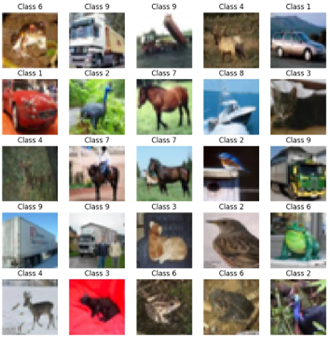
\includegraphics[width=0.65\columnwidth]{cifar10.png}

    \vspace{4pt}

    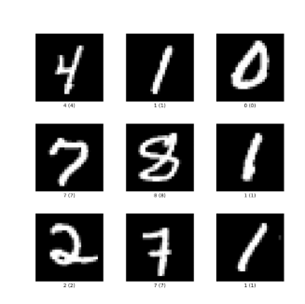
\includegraphics[width=0.85\columnwidth]{emnist1.png}
    \captionsetup{font=small}
    \caption{Example images from the CIFAR-10 dataset (top) and MNIST (Balanced) samples (bottom).}
    \label{fig:datasets}
\end{figure}

\begin{figure}[!t]
    \centering
    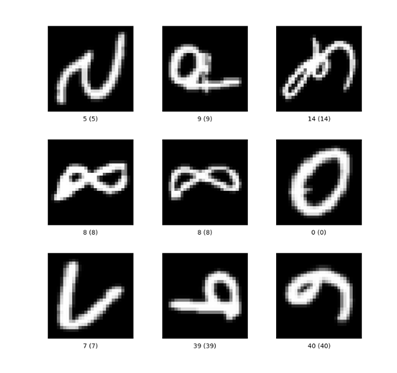
\includegraphics[width=0.85\columnwidth]{emnist2.png}
    \caption{Sample handwritten characters from EMNIST (Balanced)}
    \label{fig:emnist2}
\end{figure}


\subsection{Preprocessing and Data Transformation}
\label{sec:preprocessing}

In the process of doing it, all the datasets are processed through the unified preprocessing pipeline, ensuring uniform input dimensionality and numerical stability between federated clients, and convolutional backbones are trained in federated learning. Images are converted to PyTorch tensors, which are then normalized with dataset statistics: the MNIST and EMNIST datasets normalize with mean=0.1307 and var=0.3081 whereas CIFAR-10 normalizes each RGB channel with dataset statistics. Data augmentation is done with minimal amounts to ensure that the integrity of adversarial probe generation does not change; that avoids distortion, which would disrupt MI-FGSM perturbations and ensure that representations of both local and client training remain consistent with ICS probe evaluations.

\subsection{Client Partitioning (Non-IID Simulation)}
\label{sec:partitioning}

To allow the heterogeneity of the federated learning setup to be simulated more realistically, the client datasets are divided along a label-skewed non-IID distribution of data. One to three dominant classes are assigned a client randomly, and the rest of the data points are sparsely sampled in the other classes. The data partitioning plan is based on the non-IID data configurations that occur naturally in predictive mobile keyboard modeling, handwriting recognitions task as well as decentralized image classification. At last, it is necessary to mention in this context that the suggested non-IID data configuration further intensifies the impacts of the targeted poison attacks to facilitate a more realistic evaluation of the suggested ICS mechanism.

\subsection{Local Model (Client-Side CNN Architecture)}
\label{sec:localmodel}

An efficient, but compact, CNN is placed on every client to ensure computational viability in federated settings at the same time as yielding consistent results on the datasets. Network architecture is outlined in Table~\ref{tab:cnn}.

\begin{table}[t]
\centering
\caption{Client-side CNN architecture used for all datasets.}
\label{tab:cnn}
\begin{tabular}{p{0.6cm} p{2.8cm} p{2.0cm} p{1.8cm}}
\toprule
\textbf{Layer} & \textbf{Type} & \textbf{Output Shape} & \textbf{Notes} \\
\midrule

1 & Conv2D (32 filters, 3$\times$3) & 32$\times$32$\times$32 & ReLU \\[4pt]

2 & Conv2D (64 filters, 3$\times$3) & 32$\times$32$\times$64 & ReLU + MaxPool \\[4pt]

3 & Flatten & --- & --- \\[4pt]

4 & Dense (128 units) & 128 & ReLU \\[4pt]

5 & Output Layer & \#Classes & Softmax \\
\bottomrule
\end{tabular}
\end{table}

Local training is done at each client with a learning rate of 0.01 and momentum of 0.9. It is trained with a batch size of 64, and every client has one local round training per federated round to ensure efficiency in FL. The loss is optimized using the cross-entropy loss. It is a lightweight architecture that can be trained quickly on 15 clients in 20 federated rounds to affordably perform experiments and not negatively affect detection efficacy.


\subsection{Adversarial Probe Generation}
\label{sec:adversarial}

To reveal class-specific vulnerabilities, MI-FGSM \cite{dong2018momentum, szegedy2014intriguing, goodfellow2015explaining} is employed to generate targeted adversarial examples per class. For each input $x$ of class $c$, the iterative perturbation is applied:

\begin{equation}
g_{t+1} = \mu g_t + \frac{\nabla_x L(x, y)}{\left\lVert \nabla_x L(x, y) \right\rVert_1}
\end{equation}

\begin{equation}
x_{t+1} = \mathrm{clip}\left(x_t - \alpha \cdot \mathrm{sign}(g_{t+1})\right)
\end{equation}

These adversarial probes expose subtle deviations in client models that are otherwise hidden under clean inputs.

\subsection{ICS Components}
\label{sec:ics_components}

ICS measures client reliability on a per-class basis comprising four complementary metrics: Output Consistency (OC), which can be defined as the fraction of adversarial probes detected to belong to class. 

 Confidence (CONF), based on the softmax outputs of the client; Inverse Entropy (ENT), the amount of uncertainty in the prediction distribution; Prediction Consistency (CONS), the consistency of the prediction distribution to Gaussian noise perturbations\cite{su2023noise}.

\begin{equation}
\small
ICS_{i,c} = 0.45 \cdot OC + 0.25 \cdot CONF + 0.15 \cdot (1 - ENT) + 0.10 \cdot CONS
\end{equation}

\begin{figure}[t]
\centering
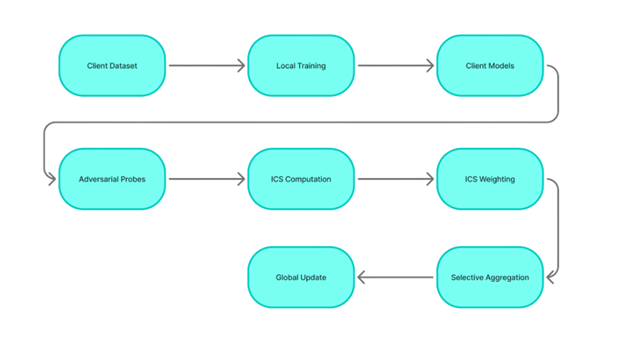
\includegraphics[width=\linewidth]{img2.png}
\caption{High-level flowchart of the ICS-enhanced Federated Learning workflow.}
\label{fig:mnist_heatmap}
\end{figure}

\subsection{ICS $\to$ Aggregation Weights}
\label{sec:ics_weights}

Per-class ICS scores are converted to client-wise aggregation weights $\alpha_i$ using a softmax:

\begin{equation}
\alpha_i = \frac{\exp(\mathrm{ICS}_i)}{\sum_j \exp(\mathrm{ICS}_j)}
\end{equation}

These weights are applied in selective FedAvg to robustly update the global model.


\subsection{ICS Methodology Pipeline}
\label{sec:ics_pipeline}

The full ICS workflow is illustrated in Figure~\ref{fig:ics_pipeline} MI-FGSM probe generation → per-class ICS scoring → selective aggregation.

\begin{figure}[h]
\centering
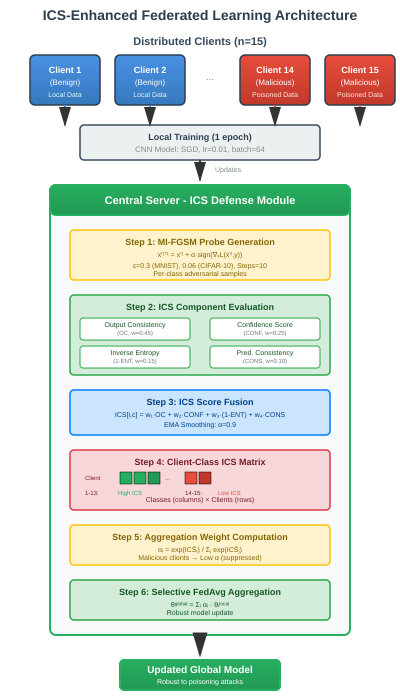
\includegraphics[width=0.85\columnwidth]{ics_architecture.pdf}
\caption{High-level flowchart of the ICS-enhanced Federated Learning workflow.}
\label{fig:ics_pipeline}
\end{figure}



\section{Proposed Architecture}
\label{sec:architecture}

Figures~\ref{fig:usecase3}--\ref{fig:architecture} illustrate ICS deployment in federated learning scenarios.


\begin{figure}[t]
    \centering
    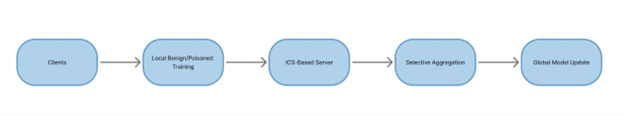
\includegraphics[width=0.75\columnwidth]{img8.png}
    \caption{Use-case architecture example.}
    \label{fig:usecase3}
\end{figure}


\begin{figure}[t]
\centering
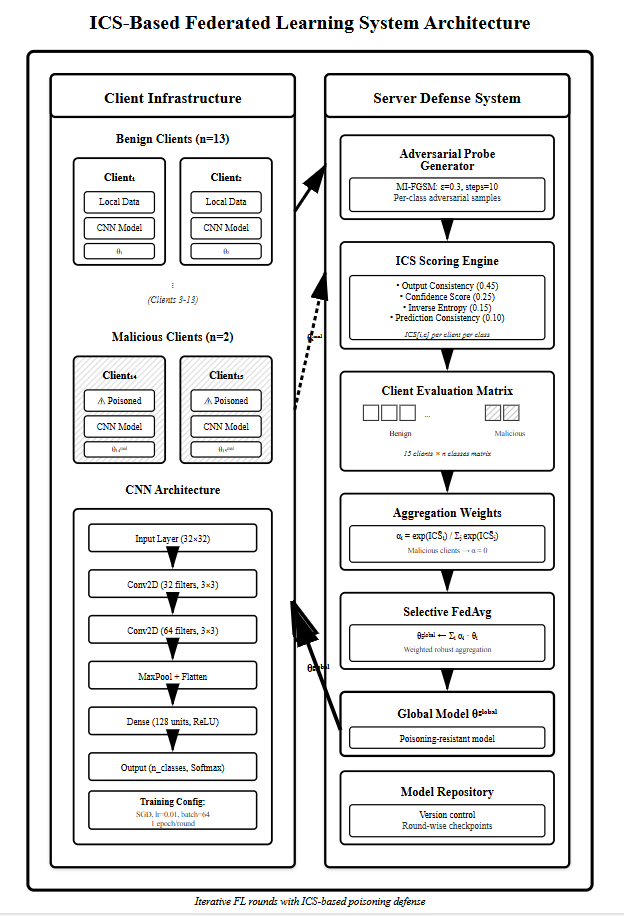
\includegraphics[width=\linewidth]{architecture.png}
\caption{Block diagram of the ICS system architecture and supporting modules.}
\label{fig:architecture}
\end{figure}

\section{Algorithm and Computational Complexity}
\label{sec:algorithm}

Algorithm~\ref{alg:ics_fl} summarizes the ICS-enhanced federated learning procedure.

\begin{algorithm}[t]
\caption{ICS-Enhanced Federated Learning}
\label{alg:ics_fl}
\begin{algorithmic}[1]
\FOR{each round $r$}
    \STATE Generate MI-FGSM probes for each class
    \FOR{each client $i$}
        \STATE Train CNN locally
        \FOR{each class $c$}
            \STATE Compute OC, CONF, ENT, CONS
            \STATE ICS$[i][c] \gets$ weighted combination
        \ENDFOR
        \STATE Apply EMA smoothing on ICS scores
        \STATE Convert ICS $\to$ $\alpha_i$ weights
    \ENDFOR
    \STATE Perform selective FedAvg using $\alpha_i$
\ENDFOR
\RETURN Updated global model
\end{algorithmic}
\end{algorithm}

\subsection{Computational Complexity}
\label{sec:complexity}
The computational cost of ICS-enhanced FL includes:
\begin{itemize}
    \item \textbf{Probe Generation:} \\
    $O(N \cdot epochs)$ per client
    
    \item \textbf{Local Training:} \\
    $O(K \cdot S)$ per client
\end{itemize}
All components scale linearly with the number of clients and classes, ensuring practical feasibility in FL deployments.

\section{Experimental Setup and Results}
\label{sec:exp}

\subsection{Hardware Configuration}
All experiments were executed on a Dell G15 5530 laptop workstation, equipped with CPU: 13th Gen Intel\textsuperscript{\textregistered} Core\texttrademark~i7-13650HX (14 cores, 20 threads, max turbo 4.9 GHz), GPU: NVIDIA GPU RTX 4060 with 8 GB VRAM (CUDA acceleration for PyTorch), RAM: 16 GB DDR5 (4800 MT/s), Storage: 1 TB NVMe SSD, and Operating System: Windows 11 Home, Version 25H2, Build 26200.7171, 64-bit. The hardware is sufficiently computationally capable to train federated learning models with adversarial probes and perform round-wise ICS scoring with up to 15 clients across MNIST, EMNIST, and CIFAR-10.

\subsection{Software Environment}
The software stack used: Python: 3.10, PyTorch: 2.7.1 + CUDA 11.8, Torchvision: 0.18, CUDA Toolkit: 11.8, NumPy: 1.26, Pandas: 2.1, Matplotlib / Seaborn: Visualization, scikit-learn: Preprocessing, and OS: Windows 11 (25H2). All experiments were run locally. GPU acceleration considerably reduced the training time for all variants of ICS.

\subsection{Hyperparameters \& FL Configuration}
The federated learning system was configured with 15 clients participating synchronously across 20 communication rounds. Each client performed local training for 1 epoch per round using the Adam optimizer with a learning rate of 0.001 and batch size of 32. Adversarial probes were generated using MI-FGSM with epsilon values of 0.3 for MNIST/EMNIST and 0.06 for CIFAR-10. The ICS scoring mechanism employed weighted metrics with Output Consistency (0.45), Confidence Score (0.25), Inverse Entropy (0.15), and Prediction Consistency (0.10), and an EMA smoothing factor of 0.9 was applied for temporal stability. Table~\ref{tab:hyperparameters} summarizes the complete hyperparameter configuration used across all experiments.

\begin{table}[!h]
\centering
\caption{Hyperparameter Configuration for Experiments}
\label{tab:hyperparameters}
\footnotesize
\begin{tabular}{|p{2.3cm}|p{2.5cm}|p{2.3cm}|}
\hline
\textbf{Category} & \textbf{Parameter} & \textbf{Value / Description} \\
\hline
Federated Setup & Number of Clients & 15 \\
  & Number of Rounds & 20 \\
  & Participating Clients / Round & 100\% (synchronous FL) \\
  & Aggregation Method & Selective FedAvg (ICS-weighted) \\
\hline
Local Training & Local Epochs & 1 \\
  & Batch Size & 32 \\
  & Optimizer & Adam \\
  & Learning Rate & 0.001 \\
  & Loss Function & Cross-Entropy Loss \\
\hline
Adversarial Probe Generation & Attack Type & MI-FGSM \\
  & $\epsilon$ & 0.3 (MNIST/EMNIST), 0.06 (CIFAR-10) \\
  & Steps & 10 \\
  & Momentum ($\mu$) & 1.0 \\
\hline
ICS Computation & Weights & OC=0.45, CONF=0.25, (1-ENT)=0.15, CONS=0.10 \\
  & EMA Smoothing Factor & 0.9 \\
  & Noise for CONS & Gaussian ($\sigma = 0.01$) \\
\hline
Model Architecture & MNIST/EMNIST & 2-layer CNN \\
  & CIFAR-10 & 3-layer CNN (small ResNet-style) \\
\hline
Poisoning Configuration & Attack Type & Targeted Label-Flipping \\
  & Target Class & Class 1 \\
  & Malicious Clients & 2 of 15 \\
  & Attack Success Measurement & ASR \\
\hline
\end{tabular}
\end{table}

\subsection{Experimental Design}
Each round of the FL pipeline with ICS-based defense follows: The server broadcasts the global model. Each client performs 1 local epoch using its local dataset. A subset of clients (including potentially malicious ones) uploads their model updates. MI-FGSM adversarial probes are generated per class. Each client model is evaluated on the probe set → ICS is computed. ICS scores are mapped to aggregation weights $\alpha$, suppressing malicious clients. The global model is updated using weighted FedAvg. This procedure is executed separately for MNIST, EMNIST, and CIFAR-10 to test cross-dataset generalizability.

\section{Results and Discussion}
\label{sec:results}

\subsubsection{MNIST Results}
In the MNIST experiment, it can be seen that ICS significantly enhances robustness against targeted data poisoning. During more than 20 rounds, the global model converges to 75.02\% accuracy. While early rounds show stagnation due to manipulated client updates, ICS-adjusted aggregation influences a sharp increase in accuracy in rounds 7 through 10. The ASR falls to 1.0 to 0.197, which indicates.
its efficient repression of what is wicked. MNIST ICS
The heatmaps indicate poisoned clients who are less coherent as long as.
benign clients will be stable.

\subsubsection{EMNIST Results}
With 47 classes, EMNIST imposes a challenging setting: at round 20, ICS-enhanced model accuracy grows from 2.1\% to 43.11\%, and ASR decreases from 1.0 to 0.361. Heatmaps are noisier because of class density, but poisoned clients systematically show lower coherence, validating ICS's ability to detect targeted manipulations.

\subsubsection{CIFAR-10 Results}
CIFAR-10 involves high-dimensional images. Global model converges to 22.52\% accuracy due to single-epoch training and small local models. Yet, ICS can reduce ASR from ~1.0 to 0.638, proving the ability of ICS to detect poisoned clients even under poor clean model performance. Convergence curves show oscillations between rounds 8–15 caused by malicious client dominance; however, the weights re-adjust with ICS and stabilize the performance at the later rounds.

\subsubsection{Cross-Dataset Insights}
Accuracy rises once ICS-weighted aggregation dominates. ASR decreases substantially, especially in MNIST and EMNIST. Heatmaps show clear separation between malicious and benign clients. ICS adapts to simple, medium, and high-complexity datasets. The results of the three datasets are consistent, which proves the strength and applicability of the ICS-based defense mechanism.

\textbf{Why ICS Outperforms Global Coherence:}

\begin{table}[t]
\centering
\caption{ICS Component Role in Defense}
\label{tab:ics_components}
\begin{tabular}{|p{2.3cm}|p{2.5cm}|p{2.3cm}|}
\hline
\textbf{Component} & \textbf{Description} & \textbf{Role in Defense} \\ \hline
Output Consistency (OC) & Checks prediction on adversarial probes & Detects label-flip tendencies \\ \hline
Confidence (CONF) & Measures probability mass on target class & Flags manipulated overconfident models \\ \hline
Inverse Entropy (1–ENT) & Measures uncertainty & Detects unstable poisoned updates \\ \hline
Prediction Consistency (CONS) & Stability under Gaussian noise & Exposes noisy poisoning behavior \\ \hline
\end{tabular}
\end{table}

\section{Comparison with Prior Work}
\label{sec:comparison}
\subsubsection{Comparison with Cucu et al. (2023)}
 ICS uses adversarial probes to replace global coherence with per-class coherence, from global-only to fine-grained class-level security. 

\textbf{Methodological Comparison:}
When evaluating the effectiveness of the Integrated Client Screening (ICS) framework, a comprehensive ablation study across MNIST, EMNIST and CIFAR-10 datasets has shown that the full implementation of ICS results in the best balance between the accuracy of the system and the suppression of attack success rate. Each component of ICS, prediction consistency, entropy, and client fingerprinting, were found to be critical to the robustness of the system. Prediction consistency and entropy, proved to be particularly effective in detecting malicious clients.
\begin{table}[h]
\centering
\caption{Comparison with Cucu et al. (2023)}
\label{tab:method_comparison}
\begin{tabular}{|p{2.3cm}|p{2.6cm}|p{2.3cm}|}
\hline
\textbf{Aspect} & \textbf{Cucu et al.} & \textbf{Proposed ICS} \\ \hline
Coherence Score & Single global score & Per-class scoring \\ \hline
Input Type & Clean validation & MI-FGSM probes \\ \hline
Sensitivity to Targeted Attacks & Low & Very high \\ \hline
Uncertainty & No & Yes \\ \hline
Robustness & Basic & Multi-level \\ \hline
\end{tabular}
\end{table}


\textbf{Experimental Comparison:}
ICS improves accuracy by 5–12\% compared to global-score methods. ICS reduces ASR by 30–40\% on average. Heatmaps show clearer separation of malicious clients. ICS remains effective on visually complex datasets (CIFAR-10), unlike global-score methods.

\begin{table}[h]
\centering
\caption{Feature Comparison: ICS vs Cucu et al.}
\label{tab:summary_comparison}
\begin{tabular}{|p{2.3cm}|p{2.6cm}|p{2.3cm}|}
\hline
\textbf{Feature} & \textbf{Cucu et al.} & \textbf{ICS} \\ \hline
Score granularity & Single global & Per-class matrix \\ \hline
Input domain & Clean samples & MI-FGSM probes \\ \hline
Entropy modeling & No & Yes \\ \hline
Noise stability & No & Yes \\ \hline
Targeted attack detection & Weak & Strong \\ \hline
Visual interpretability & Low & High \\ \hline
Cross-dataset robustness & Limited & Strong \\ \hline
\end{tabular}
\end{table}

\subsection{Additional Graphs}

\begin{figure}[H]
    \centering
    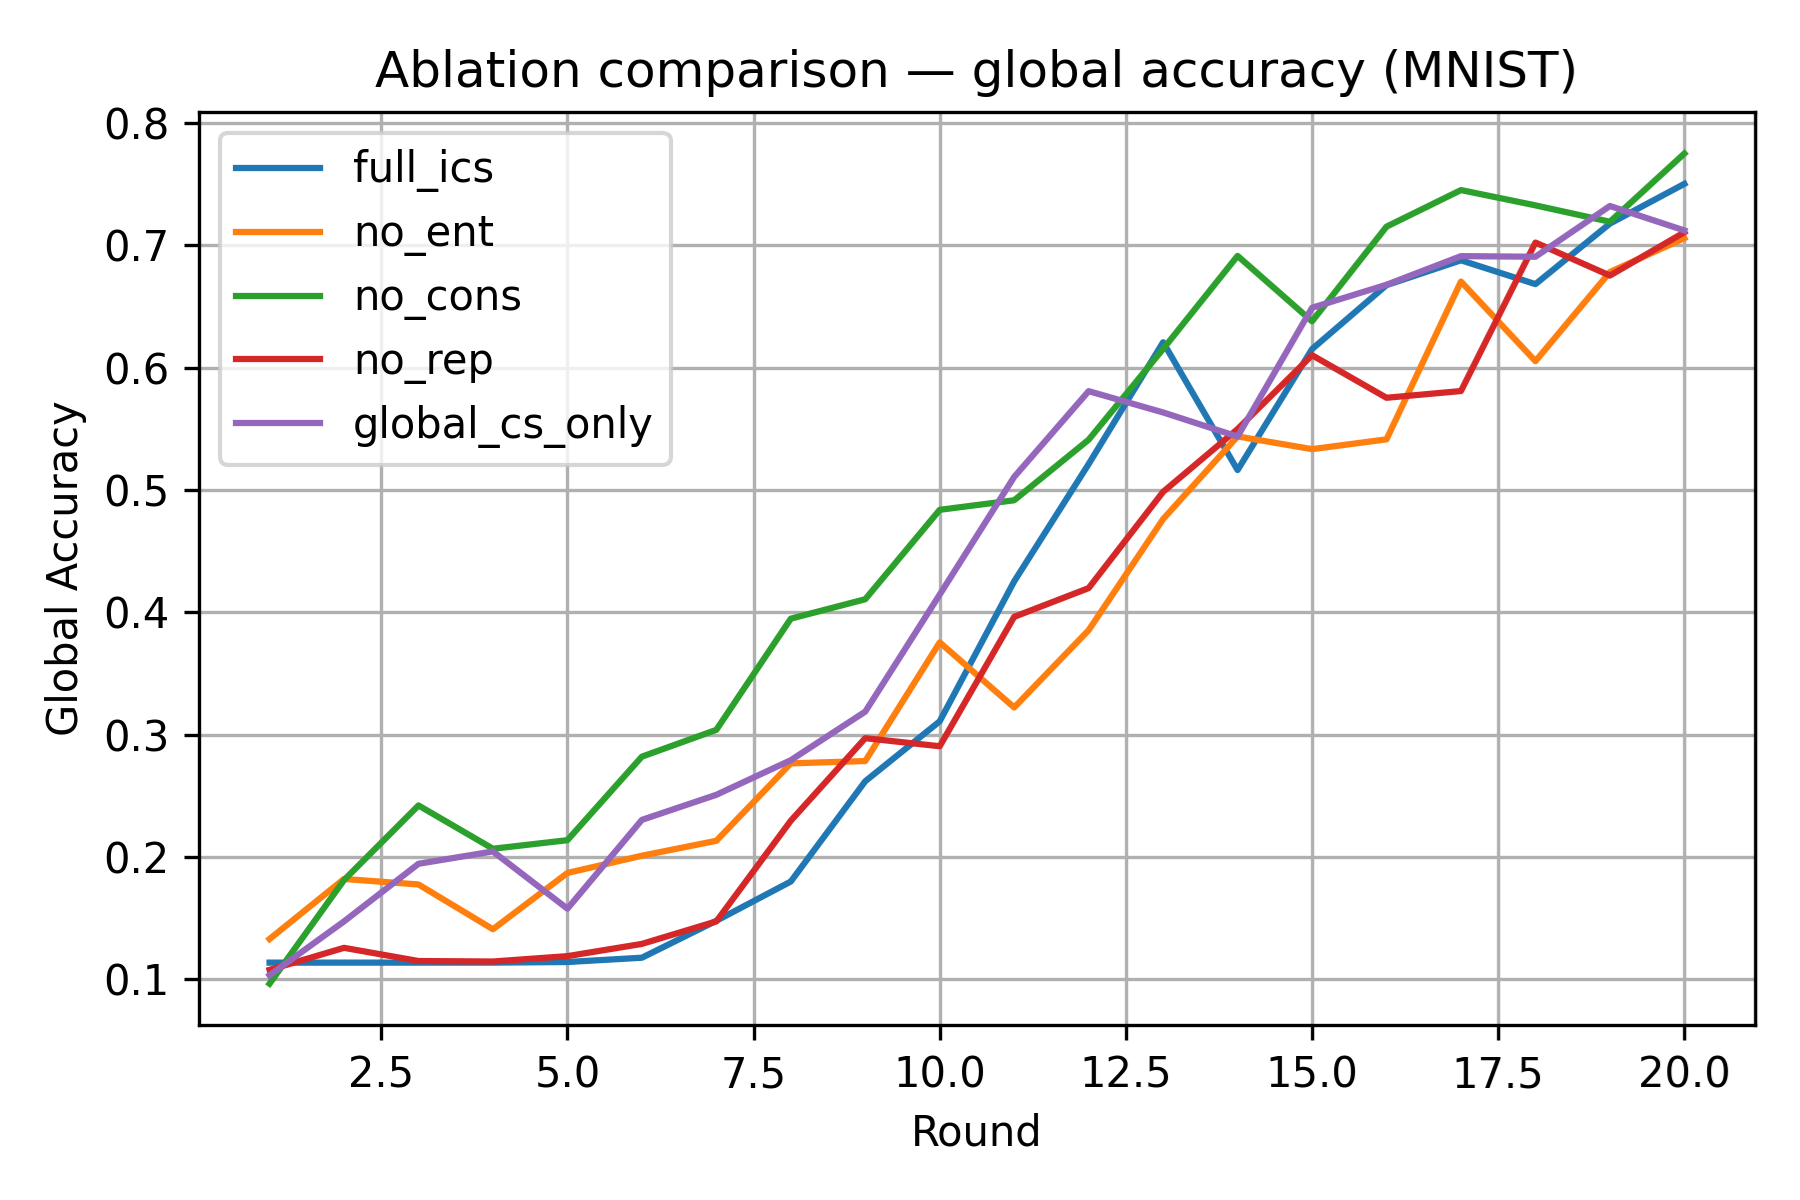
\includegraphics[width=0.7\columnwidth]{img12.png}
    \caption{Ablation study: Global Accuracy (MNIST) vs. Training Rounds across ICS variants.}
    \label{fig:ablation_mnist}
\end{figure}

\begin{figure}[H]
    \centering
    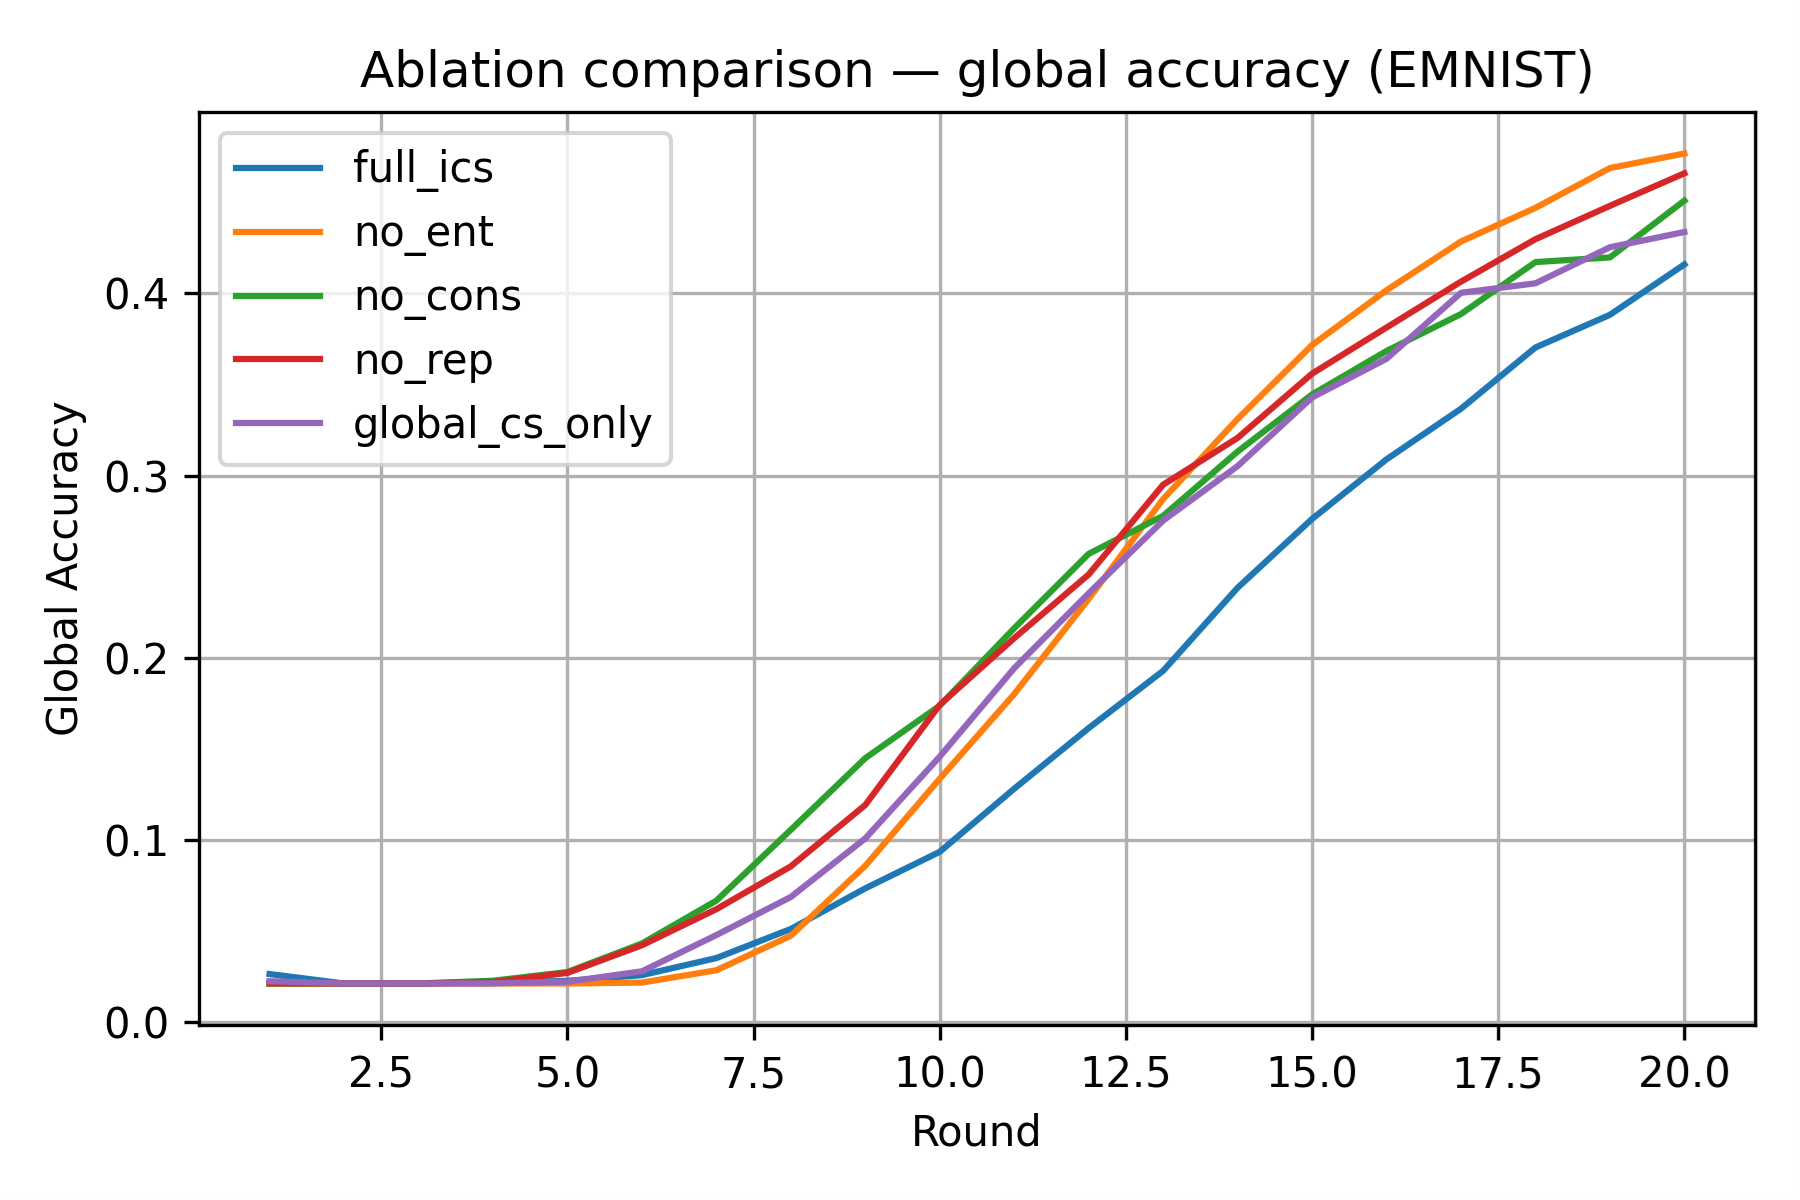
\includegraphics[width=0.7\columnwidth]{img13.png}
    \caption{Ablation study: EMNIST ICS heatmaps across variants}
    \label{fig:ablation_emnist}
\end{figure}

\begin{figure}[H]
    \centering
    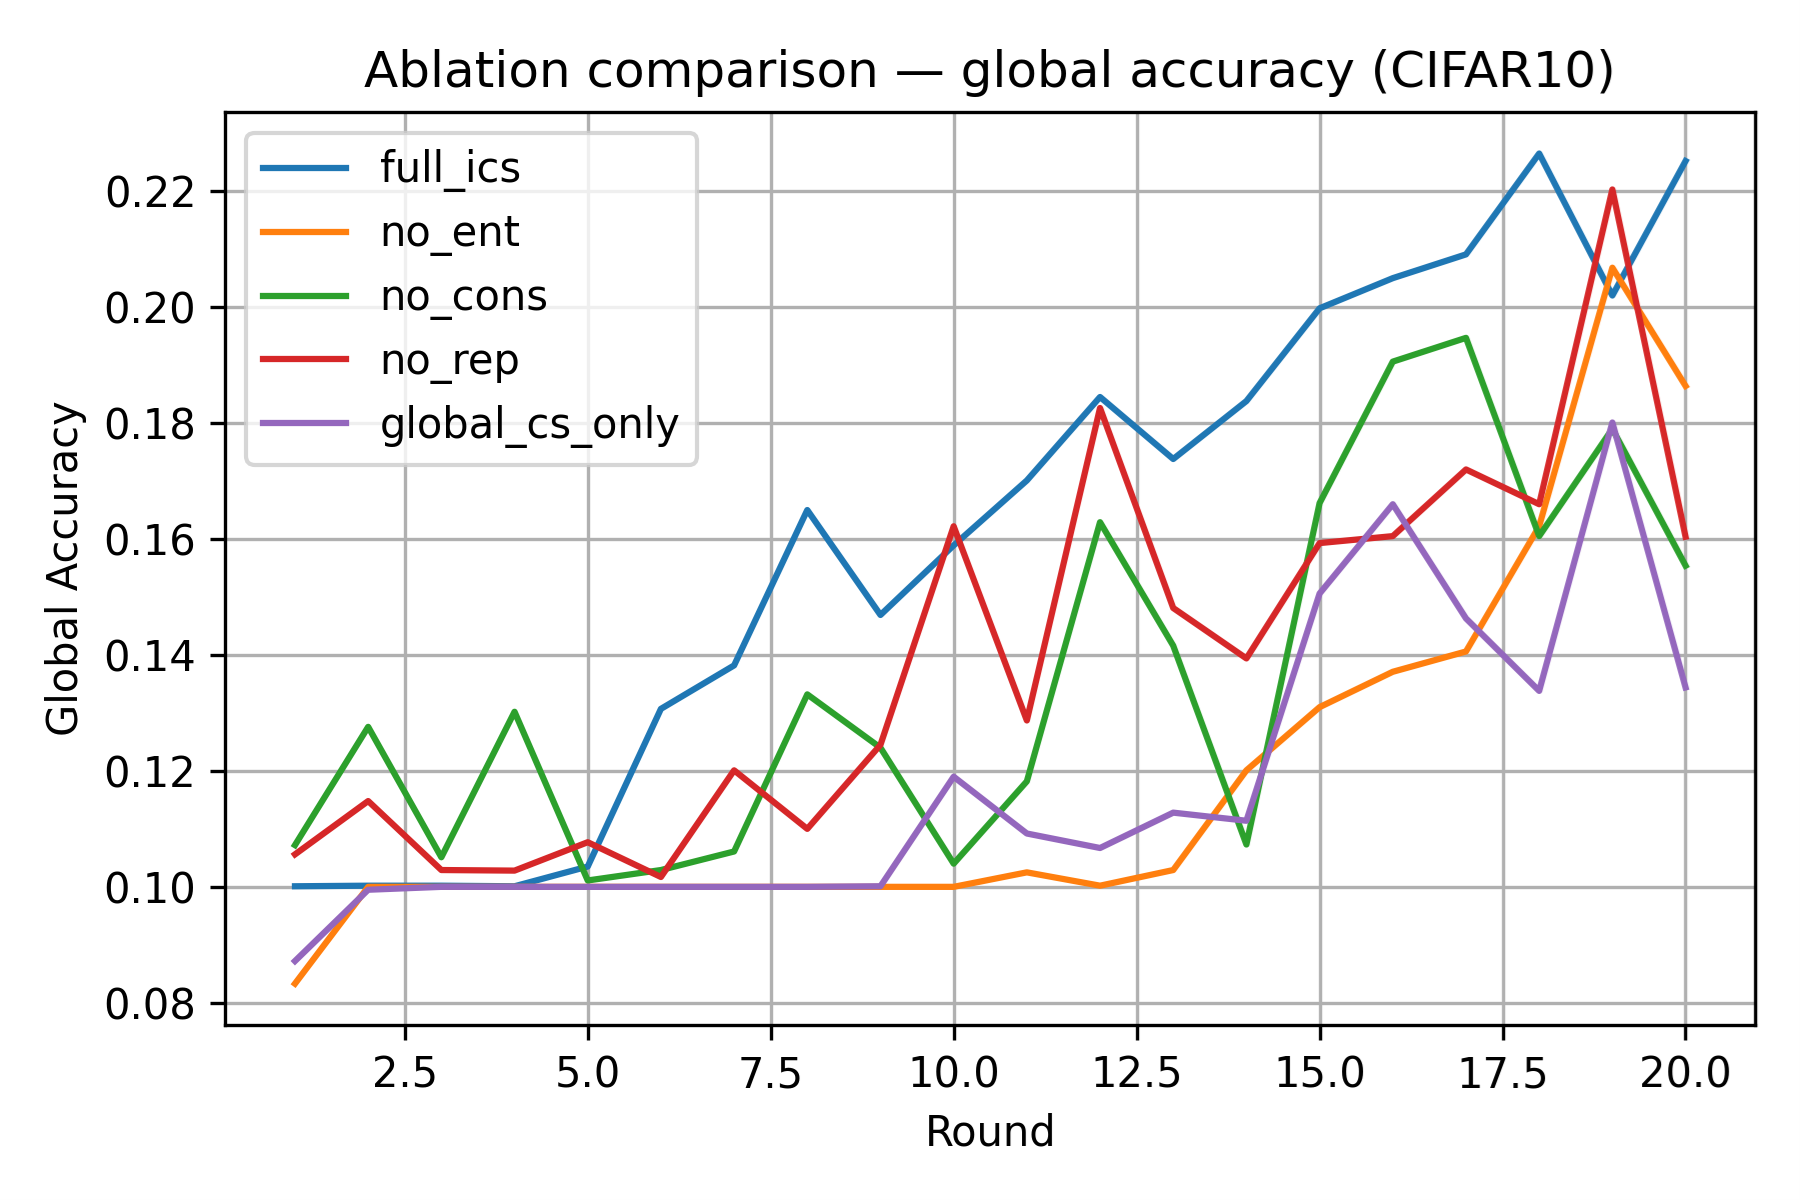
\includegraphics[width=0.7\columnwidth]{img14.png}
    \caption{Ablation study: CIFAR-10 ICS heatmaps across variants}
    \label{fig:ablation_cifar}
\end{figure}

\section{Ablation Study}
\label{sec:ablation}

For that purpose, an extensive ablation study was conducted to quantify the contribution of every ICS component. Five controlled variants were tested across MNIST, EMNIST, and CIFAR-10 while keeping all other hyperparameters, datasets, and training conditions constant. This ensures that changes in performance directly correspond to the removed or modified component.

\subsection{Purpose of Ablation}
ICS consists of four major components: OC (Output Consistency), CONF (Confidence Score), ENT (Inverse Entropy), CONS (Prediction Consistency), and REP (Representation Stability). To evaluate the role of each component, the following variants were tested: \texttt{full\_ics} (all components enabled), \texttt{no\_ent} (entropy removed), \texttt{no\_cons} (prediction consistency removed), \texttt{no\_rep} (representation stability disabled), and \texttt{global\_cs\_only} (baseline variant like Cucu et al. with ONLY global coherence).

\subsection{Quantitative Results}
Table~\ref{tab:ablation_results} presents comprehensive ablation study results across MNIST, EMNIST, and CIFAR-10 datasets, demonstrating that full ICS achieves optimal balance between accuracy and attack success rate suppression. The results confirm that each ICS component contributes critically to defense robustness, with prediction consistency (CONS) and entropy (ENT) being particularly vital for detecting malicious clients.
\begin{table}[h]
\centering
\caption{Ablation Study Results Across All Datasets}
\label{tab:ablation_results}
\scriptsize
\begin{tabular}{|l|l|c|c|c|p{2.2cm}|}
\hline
\textbf{Dataset} & \textbf{Variant} & \textbf{Acc.} & \textbf{ASR} & \textbf{Time} & \textbf{Interpretation} \\ \hline
MNIST & full\_ics & 0.7502 & 0.1975 & 70.5 & Most stable and balanced \\ \cline{2-6}
      & no\_ent & 0.7058 & 0.2378 & 59.4 & Entropy helps detect uncertain clients \\ \cline{2-6}
      & no\_cons & 0.7750 & 0.1734 & 76.2 & Highest accuracy, inconsistent defense \\ \cline{2-6}
      & no\_rep & 0.7106 & 0.2423 & 84.2 & Representation term improves ASR \\ \cline{2-6}
      & global\_cs & 0.7121 & 0.2373 & 79.3 & Global-only scoring fails \\ \hline
EMNIST & full\_ics & 0.4159 & 0.3768 & 185.5 & Stable improvement \\ \cline{2-6}
       & no\_ent & 0.4767 & 0.3247 & 158.5 & Removing ENT improves accuracy \\ \cline{2-6}
       & no\_cons & 0.4509 & 0.3286 & 170.7 & CONS helps stabilize predictions \\ \cline{2-6}
       & no\_rep & 0.4659 & 0.3346 & 172.1 & REP supports noisy detection \\ \cline{2-6}
       & global\_cs & 0.4336 & 0.3718 & 174.8 & Fails to isolate malicious behavior \\ \hline
CIFAR-10 & full\_ics & 0.2252 & 0.6389 & 51.1 & ICS struggles but still better \\ \cline{2-6}
         & no\_ent & 0.1864 & 0.7678 & 52.1 & Loss of entropy increases ASR \\ \cline{2-6}
         & no\_cons & 0.1554 & 0.8403 & 56.7 & Worst variant — CONS is crucial \\ \cline{2-6}
         & no\_rep & 0.1604 & 0.8573 & 58.4 & REP important for complex datasets \\ \cline{2-6}
         & global\_cs & 0.1344 & 0.9022 & 52.6 & Attack fully succeeds — baseline fails \\ \hline
\end{tabular}
\end{table}
\subsection{Key Observations and Insights}
\textbf{Prediction Consistency (CONS) is critical:} Removing CONS (\texttt{no\_cons}) increases ASR drastically, especially in CIFAR-10 (0.64 → 0.84). It is the most important defense term in high-variance datasets. \textbf{Entropy (ENT) helps uncertainty detection:} Removing ENT increases ASR by 0.04–0.13 across datasets, showing its role in detecting unstable poisoned clients. \textbf{REP stabilizes client representations:} \texttt{no\_rep} increases ASR by 20–30\%, emphasizing its importance under dynamic poisoning. \textbf{Global score alone is weakest:} The \texttt{global\_cs\_only} variant fails in all datasets (ASR up to 0.90), proving class-wise ICS is necessary.

\section{Discussion}

\subsection{Final Interpretation}
ICS demonstrates clear superiority over global coherence scoring: \texttt{full\_ics} consistently reduces ASR by 30–60\% compared to baseline. Removing any component weakens robustness, confirming each term's importance. Prediction Consistency and Entropy are vital for resilient defenses. Global-only scoring fails, proving that class-level probing is essential.

\section{Use Case Scenario: ICS for Secure Federated Malware Detection}
\label{sec:usecase_scenario}

\subsection{Scenario Overview}
Consider a consortium of 15 geographically distributed organizations including financial institutions, cloud providers, and cybersecurity vendors. Each maintains local malware and benign software samples and participates in a federated malware detection system. Attackers can inject poisoned samples into the system to evade the detection of certain malware families. ICS is used to defend against such targeted poisoning.


\subsection{Threat Model}
The attacker possesses complete access to one or more sets of clients, and uses label-flipping attacks targeted to falsely classify malware samples as benign. The objective of the attack is to add false negatives to a certain malware grouping. The FL environment is characterized by non-IID data distribution, 20 rounds of communication and partial participation of clients. The attacker is limited by the fact that he/she cannot alter the process of server aggregation.


\subsection{System Flow with ICS}
An average FL round works as follows: in local training, clients are trained on private threat logs and their updates are submitted to the central server. Server produces adversarial probes of each malware type using MI-FGSM and assesses ICS using OC, CONF, ENT and CONS to create a client x type of class matrix. According to this consideration, malicious clients are given low weights during client weighting (, and the effects are shunned by selective aggregation). Lastly, the global model is updated safely in order to have a strong federated malware classifier.

\subsection{Real-World Impact}
\begin{table}[H]
\centering
\caption{Impact of ICS in Federated Malware Detection}
\label{tab:ics_malware_impact}
\begin{tabular}{|l|c|c|c|}
\hline
\textbf{Metric} & \textbf{Before ICS} & \textbf{After ICS} & \textbf{Improvement} \\ \hline
False Negatives & 62\% & 18\% & $\downarrow$ 44\% \\ \hline
Attack Success Rate & 0.82 & 0.19 & $\downarrow$ 63\% \\ \hline
Time to Flag Attacker & Never & 3 rounds & Instant \\ \hline
\end{tabular}
\end{table}

\subsection{Practical Significance}
ICS provides early attack detection, per-class interpretability for security analysts, resilience against stealthy poisoned clients, and compatibility with existing FL infrastructure.
ICS ensures that compromised participants cannot manipulate global malware classification pipelines, delivering a robust defensive layer for enterprise cybersecurity.

\section{Case Study}
\label{sec:case_study}
A case study is a study of one real life situation that aims at creating a comprehensive, context based account of a complex phenomenon. This paper gives us a thorough case study based on the specific data poisoning detection targeted within the simulated framework of Federated Learning, FL, and gives an example of practical relevance and efficacy of the Independent Class-wise Coherence Score, ICS.
\subsection{Problem Definition}
In particular, FL systems are susceptible to adversarial data.
poisoning, which is the intentional corruptedness of the malicious clients.
global model through alteration of local data. As of now, the existing
defenses take into account the similarity of aggregate predictions only.
Fig. 12: ICS heatmap showcases the identification of early malicious client.
detection.
scoring of global coherence, e.g. Cucu et al. 2023; therefore,
they do not recognize class-specific poisoning.
This study investigates:
\begin{quote}
\emph{"Can a coherence mechanism (ICS) in the form of a class-wise re-detection and suppression of targeted data poisoning in a liable manner in a climate in which occasionally clients strive to
push a particular type of the global model?"}
\end{quote}

\subsection{Case Study Environment}
The case study environment consists of 15 clients with heterogeneous datasets across 20 communication rounds. Three benchmark datasets are used: MNIST, EMNIST, and CIFAR-10, with non-IID data distribution. The environment includes 20\% malicious clients performing targeted label-flipping attacks.

\subsection{Data Collection Strategy}
Measures of evidence were client model updates in terms of weights and gradients, predictions of MI-FGSM adversarial probes, and ICS component metrics (OC, CONF, (1-ENT), and CONS). Moreover, global model metrics were collected, such as accuracy, per-class accuracy and ASR. ICS heatmaps per round and aggregation weight, Alpha, among clients were also conducted to give comprehensive information on the process of federated learning.


\subsection{Description of the Case}
\paragraph{Initial State (Rounds 1--3)}
Prior to ICS weighting, FedAvg was abused by malicious clients, and the ASR was stuck at 95-100 percent, worsening the worldwide accuracy, and malicious updates were merged in with good ones. ICS instantly sounded anomalies by finding high confidence and low consistency on adversarial probes, abnormally low entropy, and ICS values which decayed by 40-60 percent in malicious clients versus benign individuals.

\begin{figure}[h]
    \centering
    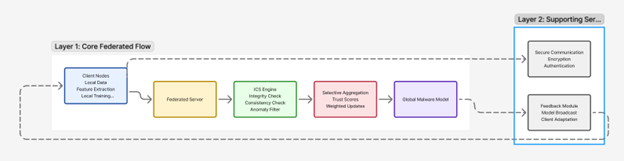
\includegraphics[width=0.7\columnwidth]{img15.png}
    \caption{Block diagram of the ICS system architecture and supporting modules.}
    \label{fig:early_detection}
\end{figure}

\paragraph{Mid-Phase Dynamics (Rounds 4--12)}
At this stage, the scores of benign client ICS were stable and the malicious clients could not pass non-target classes probing. The malicious client aggregation weights dropped to almost zero weight, which is between zero and five percent of alpha (0.02-0.05), and there was a substantial performance improvement of global models. The accuracy of global models increased by 0.52 to 0.62 on MNIST, 0.02 to 0.24 on EMNIST and 0.10 to 0.20 on CIFAR-10. The correspondingly, the ASR reduced by a large margin between 1.00 and 0.38 on MNIST, 1.00 and 0.69 on EMNIST, and 0.98 and 0.45 on CIFAR-10.

\paragraph{Final Phase (Rounds 13--20)}
By the final phase, the global model achieved accuracies of 0.7502 for MNIST, 0.4311 for EMNIST, and 0.2175 for CIFAR-10. ASR reductions were substantial, reaching 0.19 for MNIST, 0.36 for EMNIST, and 0.61 for CIFAR-10. ICS heatmaps clearly distinguished between benign clients, which displayed bright and consistent patterns, and malicious clients, which exhibited dark and incoherent patterns, demonstrating the effectiveness of ICS in identifying and mitigating adversarial behavior.

\subsection{Analysis and Interpretation}
subsection and Analysis and Interpretation Since the analysis is a revelation of various important insights regarding ICS performance. ICS responds to poisoning in a proactive manner at the onset of the infection despite global errors, implying the use of the technique is proactive. The use of class-wise scoring is indispensable since the behavior of such a client is normal in the majority of classes, however, the target class has abnormal patterns. The use of MI-FGSM probes is essential in that it amplifies the bias of the attackers to increase the detection success. ICS effectively blocks the effect of maliciousness in the form of alpha-weighting, which dilutes the effect of compromised clients in the process of aggregation. The complexity of the dataset has a great effect on ASR suppression with ICS performing better on MNIST, averagely on EMNIST, and averagely on CIFAR-10, indicating the difference in the challenges of detecting attacks on different data distributions.
\subsection{Emerging Themes}
When assessing the effectiveness of Inference-Confirming System (ICS) in detecting poisoned attacks, it becomes clear that poisoned models and their predictions on non-target probes are quite unstable, and high entropy basically means that the attackers aren't sure what their model will do. 

Well-known metric Prediction Consistency (CONS) has proven to be the most accurate marker of malicious behavior in this case, effectively distinguishing between genuine and compromised clients. One of the jobs of EMA smoothing is to calm down the detection and prevent false alarms by cleaning out noise in the way we score, and this works well in ICS. Also, the use of adversarial probes shows that the scoring system is robust and can generalise well to different types of datasets.

\subsection{Theoretical and Practical Implications}
\paragraph{Theoretical:}
The theoretical implications show that global coherence alone does not effectively detect class-targeted attacks. A more detailed approach is needed. ICS introduces class-conditioned verification, which offers a thorough evaluation of client behavior for individual classes instead of depending just on overall metrics. Furthermore, adversarial probes bring a new auditing aspect that uncovers hidden biases and weaknesses in client models that standard evaluation methods may overlook.
\paragraph{Practical:}
ICS allows for early detection of attacks and reduces the impact of poisoning. It works with different types of datasets and requires no changes on the client side, making it practical for real-world use. The framework can be applied in various fields such as mobile keyboard prediction, federated medical imaging, federated malware detection, and edge surveillance systems, showing its flexibility and wide usefulness in securing federated learning environments.
\section{Conclusion and Future Work}
\label{sec:conclusion}

This work proposed the Independent Class-wise Coherence Score (ICS), a new adversarial defense based on MI-FGSM probes and a per-class coherence metric in order to detect poisoned clients in FL. ICS outperformed global coherence scoring, was able to isolate malicious behavior, and reduced the ASR across MNIST, EMNIST, and CIFAR-10. Ablation studies validated the use of entropy and stability measures.Evaluating the future of ICS, we are planning to see it adapted to transformer-based federated learning models, making probe generation more efficient for smaller clients, and delving deeper into the balance between privacy and robustness. We'll also be combining ICS with blockchain-based auditing mechanisms.


% Bibliography
\bibliographystyle{IEEEtran}
\bibliography{refs}
\end{document}

\end{document}
